\documentclass[tikz,border=2pt]{standalone}
\usepackage{amsmath}
\usepackage{pgfplots}
\pgfplotsset{compat=1.18}
\usetikzlibrary{arrows.meta}
\begin{document}
% A nested call is evaluated inside out: round(mean(c(1, 2, 4)), 1)
% c() builds the vector, mean() gives 2.333333, round(., 1) gives 2.3.
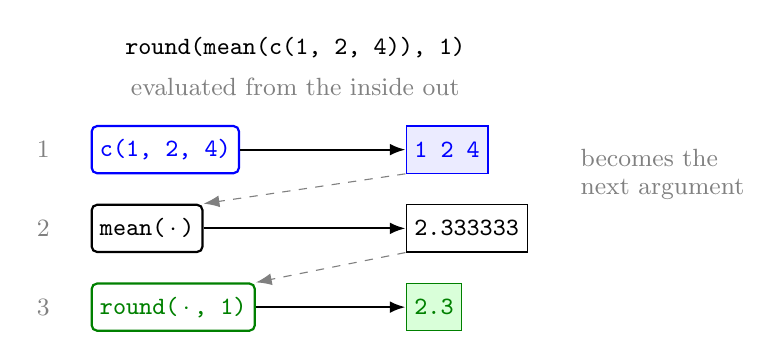
\begin{tikzpicture}[font=\small, >={Latex[length=2mm]},
  call/.style={draw, thick, rounded corners=2pt, minimum height=6mm, inner sep=3pt, font=\small\ttfamily},
  val/.style={draw, minimum height=6mm, inner sep=3pt, font=\small\ttfamily}]
  \node[font=\small\ttfamily] at (2.6,3.3) {round(mean(c(1, 2, 4)), 1)};
  \node[gray] at (2.6,2.8) {evaluated from the inside out};
  \node[gray] at (-0.6,2) {1};
  \node[gray] at (-0.6,1) {2};
  \node[gray] at (-0.6,0) {3};
  \node[call, blue, anchor=west] (c1) at (0,2) {c(1, 2, 4)};
  \node[val, blue, fill=blue!8, anchor=west] (v1) at (4,2) {1 2 4};
  \node[call, anchor=west] (c2) at (0,1) {mean(\,$\cdot$\,)};
  \node[val, anchor=west] (v2) at (4,1) {2.333333};
  \node[call, green!50!black, anchor=west] (c3) at (0,0) {round(\,$\cdot$\,, 1)};
  \node[val, green!50!black, fill=green!15, anchor=west] (v3) at (4,0) {2.3};
  \draw[->, thick] (c1) -- (v1);
  \draw[->, thick] (c2) -- (v2);
  \draw[->, thick] (c3) -- (v3);
  \draw[->, gray, dashed] (v1.south west) -- (c2.north east);
  \draw[->, gray, dashed] (v2.south west) -- (c3.north east);
  \node[gray, anchor=west] at (6.1,1.9) {becomes the};
  \node[gray, anchor=west] at (6.1,1.5) {next argument};
\end{tikzpicture}
\end{document}
